\documentclass[fyp]{socreport}
\usepackage{hyperref}
\usepackage{graphicx} % to insert images
\usepackage{float}
%%% code block setups
\usepackage[newfloat]{minted}
\usepackage{xcolor} % to access the named colour LightGray
\definecolor{LightGray}{gray}{0.9}
\usepackage{caption}
\newenvironment{code}{\captionsetup{type=listing}}{}
\SetupFloatingEnvironment{listing}{name=Code}
%%% code block setups
\usepackage{fullpage}
\usepackage{multirow}
\usepackage{longtable}
\usepackage{amsmath}

\begin{document}
\pagenumbering{roman}
\title{Competition Platform for AI Tasks}
\author{Tan Yuanhong}
\projyear{2021/22}
\projnumber{H247080}
\advisor{Dr. Akshay Narayan, Prof. Leong Tze Yun}
\deliverables{
	\item Report: 1 Volume
	\item Source Code: 1 Git Repository
}
\maketitle
\begin{abstract}
Entering the second decade of the 21st century, machine learning and artificial intelligence is the new must-have for computer science education. However, while the data-oriented tasks like classification and regression have well-adopted platforms such as Kaggle, simulation-oriented tasks that are most common for reinforcement learning (RL) algorithms are yet to have a feature-complete online judging solution. This project aims to build a complete solution that is extensible, scalable, and easy-to-use. It covers four critical components of judging RL algorithms: a simulation environment framework, an auto-grading framework, a scalable and secure sandbox for arbitrary code execution, and finally a modern web application as the entry point. Besides a comprehensive documentation and many quality-of-life new features and improvements, this project greatly improves the performance of existing internal platform with a task queue system that not only distributes tasks fairly, but also dynamically adapts to the load of each worker node thanks to its resource awareness. Experimental results show that the new system provides fair task distribution among worker nodes and nearly three times of resource utilization improvement over aiVLE 1.0 ($>90\%$ vs $\approx 30\%$).

\begin{project-nature}
	Implementation, Experimentation, Simulation
\end{project-nature}
\begin{keywords}
    \item Artificial Intelligence
	\item Machine Learning
\end{keywords}
\begin{implement}
	Ubuntu 20.04, Firejail 0.9.68, Python 3.8, Django 4.0, Celery 5.2
\end{implement}

\end{abstract}

% \begin{acknowledgement}
%   I would like to thank my friends, families and advisors.
%   Without them, I would not have be able to complete this project.
% \end{acknowledgement}

\listoffigures 
\listoftables
\tableofcontents 

\chapter{Introduction}

With the increasing popularity in both artificial intelligence (AI) research and industry application, more and more institutions are considering AI education as an integral part of their computer science or even general education curriculum. However, in spite the algorithmic nature of AI education, there is surprisingly few platforms and tools to host AI competitions/assignments and automatically grade the submissions. Unlike traditional algorithm and data structure courses that have many online judges available (to name a few, \href{https://codeforces.com/}{Codeforces}, \href{https://open.kattis.com/}{Kattis}, \href{https://onlinejudge.org/}{UVa Online Judge}), AI courses often rely on arbitrary grading scripts or in-house solutions to host their assignments/contests. There are well-known data science competition platforms like \href{https://www.kaggle.com/}{Kaggle} that are suitable for prediction/classification tasks, but the area of reinforcement learning (RL) tasks \footnote{To be precise, here tasks mean environments that are typically used for RL algorithms. The differentiating characteristic of such tasks is that they are interactive (in contrast to comparing the output against the ground truth like what Kaggle and other traditional OJs do).} remains surprisingly untouched. Therefore, this project tries to fill the gap of evaluating algorithms that solve interactive tasks. We aim to provide a complete solution from building RL \footnote{Technically the evaluation model we use is suitable for almost all AI/ML tasks (including classification and regression), but we will focus on RL first since we already have Kaggle for classification/regression tasks.} environments, writing test cases, to eventually hosting these tasks on a massively scalable platform.

\chapter{Project Objective}
\label{ch:project-objective}
\section{Problem Statement}
\label{s:project-objective-problem-statement}
The goal of this project is to provide a complete solution for RL algorithm evaluation that is extensible, scalable, and easy-to-use. It consists of four tightly integrated components (collectively called aiVLE 2.0):

\begin{enumerate}
    \item aiVLE\footnote{aiVLE is name for the grading system currently used in CS4246, more details about the old aiVLE (aiVLE 1.0) are covered in Section~\ref{ch:literature-review-related-work-ai-competition-platforms}} Gym: An OpenAI Gym \parencite{openai-gym} compatible RL environment framework with agent-environment separation and official support for multi-agent tasks.
    \item aiVLE Grader: An auto grading framework for aiVLE Gym tasks.
    \item aiVLE Worker: A security sandbox to execute arbitrary code submissions safely in a resource restricted environment. And a massively scalable worker client for evaluation.
    \item aiVLE Web: A web application for hosting RL competitions.
\end{enumerate}

\section{Motivation}
\label{s:project-objective-motivation}
Courses like CS4246, which teach AI, and are different from traditional programming/algorithm courses, need a system to automate the process of collecting and evaluating programming assignments on AI tasks. aiVLE 1.0 provides instant feedback on programming assignments that require varied computational power such as GPU or other specialized processing units. However, as mentioned in Section~\ref{ch:literature-review-related-work-ai-competition-platforms}, aiVLE 1.0 has many pain points. For example, it lacks extensibility (e.g., does not support multi-agent task), scalability (e.g., no concurrency safety for many workers), and documentation for more courses to make use of the platform. As for another similar platform called Botzone~\parencite{botzone}, although it is built for external users, limitations like no GPU support and no common interface make it infeasible for many tasks.

Secondly, an open source RL competition platform with good documentation and software engineering best practices has potential impact beyond education purposes. On the one hand, such a platform could also be useful for benchmarking AI algorithms – the consistency required for grading assignments is perfect for comparing research as well. On the other hand, examples like AlphaGo~\parencite{alphago} proves the effectiveness of combining supervised learning from past match data with unsupervised RL – match history collected on the platform could be useful for training models for corresponding tasks. 

Lastly, there is demand for such a platform. Both CS3243 and CS4246 have assignments on RL algorithms, and many non-RL tasks such as brute force or informed search, satisfiability problems, can be solved using similar execution loops. It is a safe bet that such a platform will benefit many AI courses (including CS2109S and CS3244) by using it alongside platforms like Kaggle to cover most AI algorithm evaluation scenarios.

\section{Roadmap}
\label{s:project-objective-roadmap}
There are three stages planned for this project. During the first semester, we delivered satisfactory results for the first two stages. During the winter break, we conducted \hyperref[ch:deployment-and-testing]{real-world deployment and testing} to evaluate the feasibility of advancing the project to the third stage. During the second semester, we focused on fixing problems found during the test, and delivering features as mentioned in the third stage.

\subsection{Stage 1: Framework}
Before developing the web platform for hosting the competitions, we first need frameworks for 1) creating environment and 2) evaluating agent’s performance – \hyperref[ch:aivle-gym]{aiVLE Gym} and \hyperref[ch:aivle-grader]{Grader} respectively. These frameworks are independent from the web platform, therefore could be used separately for other education or research purposes as well.
Besides being a platform-independent framework, a security sandbox, \hyperref[ch:aivle-worker]{aiVLE Worker}, is also necessary for hosting competitions. These three frameworks will be implemented in the mentioned order as the latter have dependency on the former.

\subsection{Stage 2: Platform}
With the frameworks ready, the second stage is to have \hyperref[ch:aivle-web]{a web platform} that achieves basic online judge functionality, which includes but is not limited to: 1) user registration and authentication, 2) creating/joining courses, 3) creating/modifying/submitting tasks, 4) showing the evaluation result. The target of this stage is to have a \emph{minimum viable product} that CS4246 can use to host single-agent assignments with GPU-accelerated evaluation.

\subsection{Stage 3: Advanced Solution}
Stage 1 and 2 provide a solid foundation for further extension and exploration, but primarily focus on delivering features that are necessary (thus \textbf{minimally} viable) for CS4246 teaching. Stage 3 aims to further extend the use case of our web platform. First, we will perform a real-world deployment and stress test of the system, which 1) validates the stability and performance gain of the new architecture, and 2) irons out unexpected behaviors and discrepancies in the deployment instructions. Second, we will improve the documentation of the source code and use cases, which is crucial for the maintainability and upgradability of this project. Lastly, we will add advanced features that are so-called ``quality-of-life updates''\footnote{There are also many other nice-to-have features that did not appear in this report, like more user-friendly frontend and course administration tools. To keep the report relatively concise, we only cover features that are deemed significant or technically challenging.} but are achievable within the time constraint (e.g., Sections \ref{ss:aivle-worker-resource-awareness} for resource awareness, \ref{ss:aivle-web-load-balancing} for load balancing).
\chapter{Design and Implementation}
\label{ch:design-and-impl}
Following the nomenclature defined in Section~\ref{ch:literature-review-related-work-ai-competition-platforms}, we will call the new system aiVLE 2.0 henceforth. Do note that aiVLE 2.0 also refers to the new system architecture as a whole~–~every sub-project has an independent versioning that does not necessarily share the major revision number 2 because components like aiVLE Gym and aiVLE Grader do not exist in aiVLE 1.0. As mentioned in Section~\ref{s:project-objective-problem-statement}, there are four components in aiVLE 2.0: aiVLE Gym, Grader, Worker and Web. As a high-level overview, Figure~\ref{fig:architecture-overview} shows the relationship between the components: the system can be roughly divided into client-side (where users write and run the agents locally) and server-side (where the platform hosts the competition and evaluates the submissions in a security sandbox). On the client side, we have \textbf{aiVLE Gym} (Section~\ref{ch:aivle-gym}) responsible for simulation. \textbf{aiVLE Grader} (Section~\ref{ch:aivle-grader}) calls the agent implementation to interact with the environment and record the simulations. On the server side, student submissions are evaluated inside the security sandbox of \textbf{aiVLE Worker} (Section~\ref{ch:aivle-worker}), ensuring fair resource allocation and secure code execution. We also have a worker cluster consisting of many worker nodes, communicating with \textbf{aiVLE Web} (Section~\ref{ch:aivle-web}) in an orchestrated manner. This cluster is designed to be fault tolerant and massively scalable. And of course, aiVLE Web also provides a frontend that you can access from a browser.

\begin{figure}[H]
    \centering
    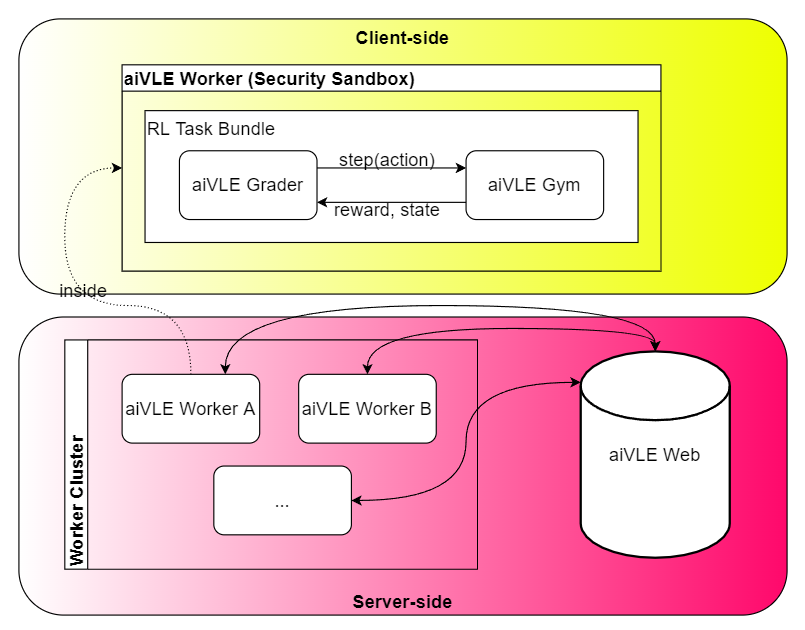
\includegraphics[width=0.9\textwidth]{images/architecture-overview.png}
    \caption{aiVLE 2.0 Architecture Overview}
    \label{fig:architecture-overview}
\end{figure}

In this chapter, we will discuss about the design and implementation of all these four components in detail, the order of which is also the chronological order of development: the later components may have dependencies on earlier ones, and the earlier components generally\footnote{Strictly speaking, aiVLE Worker does not depend on aiVLE Web, but when it is used as a worker client on top of a security sandbox, although it will startup normally, without aiVLE Web to push evaluation jobs into the task queue, the worker client is meaningless. So we used ``generally'' here just to be precise.} do not depend on the later ones. For example, aiVLE Gym can be used as general-purpose multi-agent environment framework outside of the aiVLE 2.0 platform.

\section{aiVLE Gym - Separating Agents from Environment}
\label{ch:aivle-gym}
I have released a stable version of aiVLE Gym with all planned features implemented. \href{https://github.com/edu-ai/aivle-gym}{The source} consists of $\sim$1K lines of code, including several example environments and full documentation. The package is published to PyPI  (\href{https://test.pypi.org/project/aivle-gym}{https://test.pypi.org/project/aivle-gym}) so that aiVLE Gym can be installed and imported like any other Python package. A brief user guide can be found at \href{https://edu-ai.github.io/aivle-docs/user-guide/aivle-gym/}{https://edu-ai.github.io/aivle-docs/user-guide/aivle-gym/}.

\subsection{Motivation}
aiVLE Gym makes multi-agent competition possible by separating agents from the environment. In a two-agent OpenAI Gym\parencite{openai-gym} task, we write agent code as shown in Code~\ref{code:two-agent-example}:

\begin{code}
\begin{minted}[frame=lines,framesep=2mm,baselinestretch=1.2,bgcolor=LightGray,fontsize=\footnotesize,linenos,samepage]{python}
env = gym.make("PongDuel-v0") # Two-player Ping Pong game

for ep_i in range(100):
    done_n = [False for _ in range(env.n_agents)]
    ep_reward = 0
    obs_n = env.reset()
    env.render()
    while not all(done_n):
        action_0 = decide_0(obs_n[0], reward_n[0])
        action_1 = decide_1(obs_n[1], reward_n[1])
        action_n = [action_0, action_1]
        obs_n, reward_n, done_n, info = env.step(action_n)
        ep_reward += sum(reward_n)
        env.render()
    print('Episode #{} Reward: {}'.format(ep_i, ep_reward))

env.close()
\end{minted}
\captionof{listing}{OpenAI Gym agent example}
\label{code:two-agent-example}
\end{code}

Note that in a multi-agent scenario, \texttt{observation}, \texttt{reward} and \texttt{done} are all vectors - each element corresponds to one of the agents. Similarly, when you call \texttt{env.step()}, you should provide \texttt{action}s for every agent in this simulation. Such design is acceptable when we perform these multi-agent experiments offline in a controlled manner. However, in a competition setting, when it comes to multi-agent tasks, you cannot make decisions for your opponent agents. Therefore, separating agents from the environment simulation is necessary. From the perspective of each agent, it is just like a single-agent environment – the only difference is that the environment is affected by actions taken by other agents as well. Figure~\ref{fig:opanai-gym-multi-arch} and Figure~\ref{fig:aivle-gym-multi-arch} show the architectural differences between \emph{OpenAI} Gym and \emph{aiVLE} Gym (each colored box represents a separate process; solid arrows represent inter-process or network communication):
\begin{figure}[H]
    \centering
    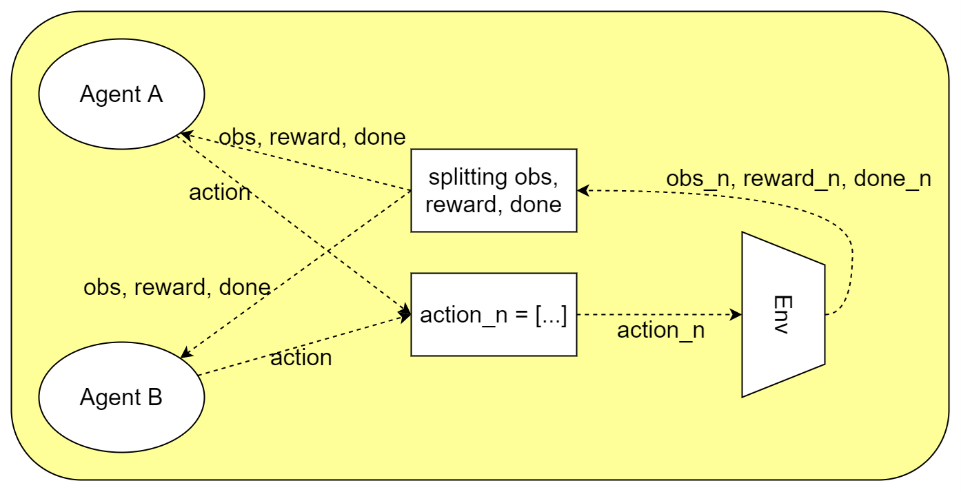
\includegraphics{images/opanai-gym-multi-arch.png}
    \caption{Multi-agent Architecture in OpenAI Gym}
    \label{fig:opanai-gym-multi-arch}
\end{figure}
\begin{figure}[H]
    \centering
    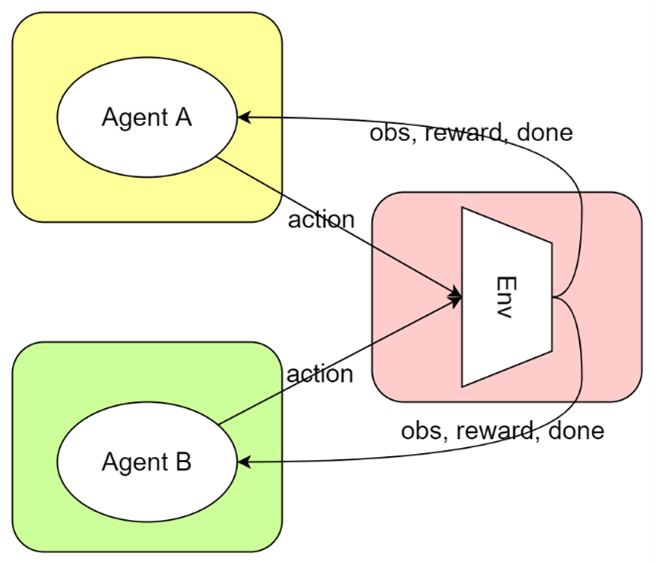
\includegraphics{images/aivle-gym-multi-arch.png}
    \caption{Multi-agent Architecture in aiVLE Gym}
    \label{fig:aivle-gym-multi-arch}
\end{figure}

\subsection{Design Goal}
Unless mentioned otherwise, all design goals in this chapter are achieved in the released implementation. 

The design goal of aiVLE Gym is to keep full compatibility with OpenAI Gym on the agent side. On the environment side, it lets you convert from existing OpenAI Gym environments with minor adaptation. More specifically:

In single-agent case, on the agent side, traditional environment (simulation happens within agent process) and aiVLE environment (simulation happens outside of agent process) should be interchangeable. On the environment side, author can reuse existing OpenAI Gym compatible environment by implementing a serializer that serializes \texttt{action}, \texttt{observation}, and \texttt{info} to JSON compatible objects (Code~\ref{code:aivle-gym-serializer}).

\begin{code}
\begin{minted}[frame=lines,framesep=2mm,baselinestretch=1.2,bgcolor=LightGray,fontsize=\footnotesize,linenos,breaklines,samepage,highlightlines={7-11,14-15}]{python}
class CartPoleEnvSerializer(EnvSerializer):
    def action_to_json(self, action):
        return action
    def json_to_action(self, action_json):
        return action_json

    '''Because numpy.array objects are not JSON-serializable by default,
    we provide custom methods to marshal/unmarshal observations.
    As shown in this example, if action/observation/info are JSON-serializable
    to begin with, you just return the original value.
    '''
    def observation_to_json(self, obs):
        return obs.tolist()
    def json_to_observation(self, obs_json):
        return numpy.array(obs_json)

    def info_to_json(self, info):
        return info
    def json_to_info(self, info_json):
        return info_json
\end{minted}
\captionof{listing}{aiVLE Gym Environment Serializer Example}
\label{code:aivle-gym-serializer}
\end{code}

In multi-agent case, on the agent side, the APIs behaves just like normal single-agent OpenAI Gym environment. On the environment side, author can reuse existing ma-gym environment~\parencite{magym} by implementing a serializer along with several metadata fields. 

\subsection{Agent-Environment Communication}
\label{ss:agent-env-communication}
Since agents and environment are separated, we need an inter-process communication channel between them. aiVLE Gym uses a lightweight yet high-performance messaging library ZeroMQ~\parencite{zeromq}, which has comprehensive support for many synchronous and asynchronous messaging patterns that are essential to this project. There are two primary challenges for multi-agent tasks when it comes to agent-environment communication:
\begin{enumerate}
    \item The judge should receive and respond to requests asynchronously - it needs to wait for all agents' actions before stepping forward in the environment, then decide on what observations/rewards to respond to each of the agents.
    \item Certain operations (e.g., resetting the simulation) must be performed strictly once for each episode, but since each agent will initialize the episode on their own, judge-side will unavoidably receive multiple requests.
\end{enumerate}

To summarize, the judge-side environment needs to implement a ``barrier'' synchronization mechanism that not only realizes synchronous rendezvous of agent requests, but also performs additional tasks upon the ``first-comer'' and ``last-leaver''. 

Therefore, we propose the deterministic finite automaton (DFA) as shown in Figure~\ref{fig:aivle-gym-multi-dfa}:
\begin{figure}[H]
    \centering
    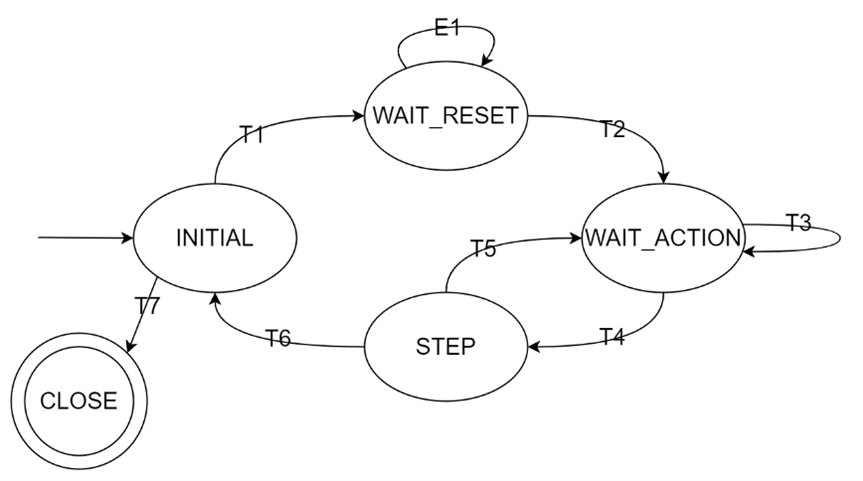
\includegraphics{images/aivle-gym-multi-dfa.png}
    \caption{aiVLE Gym Multi-agent Environment Communication Automaton}
    \label{fig:aivle-gym-multi-dfa}
\end{figure}

This DFA is key to keeping complicated communication details transparent to both agent and environment logic – both can write common synchronous code while the framework deals with the underlying asynchronous logic. Details of this DFA and messaging patterns involved can be found in the Appendix~\ref{as:aivle-gym_dfa}.

\section{aiVLE Grader - Evaluating Agents Using Test Suites}
\label{ch:aivle-grader}
I have released a stable version of aiVLE Grader with support for 1) OpenAI Gym, 2) aiVLE Gym single-agent, and 3) aiVLE Gym multi-agent environment. The codebase consists of $\sim$600 lines of framework code and $\sim$300 lines of example test suites for all three supported use cases. Similar to aiVLE Gym, the package is released to PyPI  (\href{https://test.pypi.org/project/aivle-grader/}{https://test.pypi.org/project/aivle-grader}) for in-production usage. A brief user guide can be found at \href{https://edu-ai.github.io/aivle-docs/user-guide/aivle-grader/}{https://edu-ai.github.io/aivle-docs/user-guide/aivle-grader/}.

\subsection{Design Goal}
Unlike competitive programming style problems or machine learning prediction tasks, evaluating RL agents is much more complicated than comparing students’ output against a standard answer. Fortunately, with the common programming interfaces provided by OpenAI/aiVLE Gym, we may create a framework that standardizes/modularizes the initialization, execution, and conclusion of RL agent evaluation. The ultimate goal of this framework, when writing a grader for agents in any OpenAI/aiVLE Gym environment, is to:
\begin{enumerate}
    \item Make the built-in components complete enough such that for most use cases using built-in ones would be sufficient.
    \item Make each component self-contained without complicated inter-dependencies (i.e., following the single responsibility principle) when writing a custom component.
\end{enumerate}

\subsection{Key Abstractions}
There are three key abstractions to aiVLE Grader: \textit{agent}, \textit{evaluator}, and \textit{test case} as summarized in Figure~\ref{fig:aivle-grader-class}.

\begin{figure}[H]
    \centering
    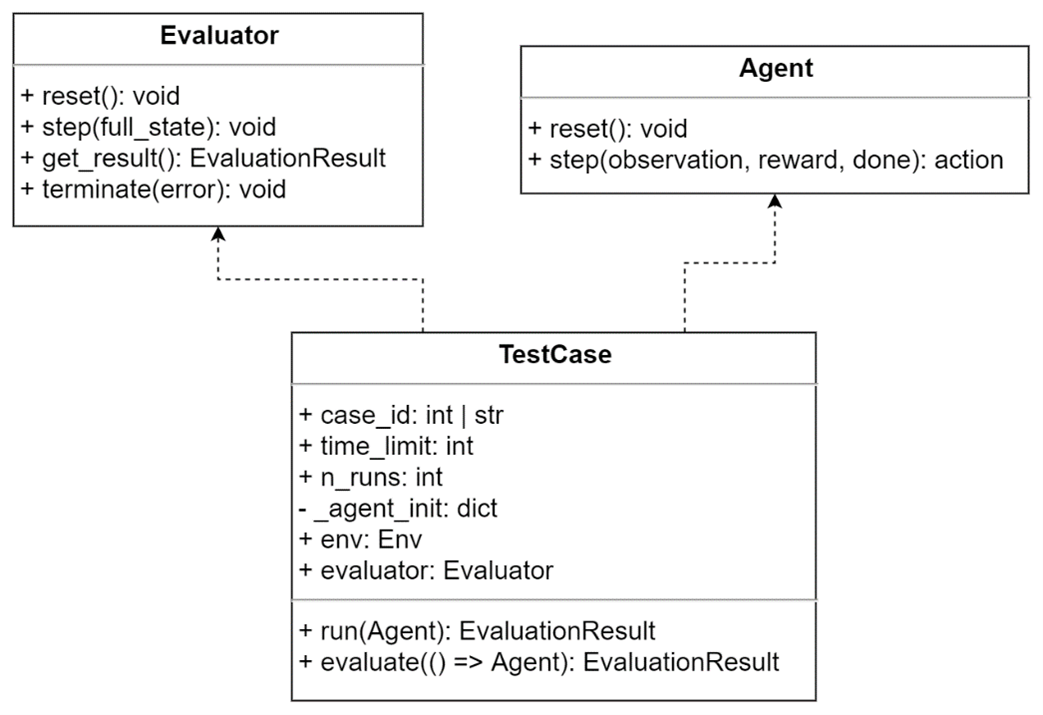
\includegraphics{images/aivle-grader-class.png}
    \caption{Class Diagram for aiVLE Grader}
    \label{fig:aivle-grader-class}
\end{figure}

\textit{Agent} only has two methods: \texttt{reset} to reset internal states, \texttt{step} to return an action from provided observation. It is flexible enough to allow agents to memorize the history, whilst restrictive enough to prohibit agents from modifying the inner-workings of the environment.

\textit{Evaluator} records the entire execution process and produces a score when the session terminates. It utilizes the common pattern of most RL tasks (see Figure~\ref{fig:obr-loop}): each session consists of many episodes, and each episode consists of many concrete steps. By inserting hook functions to these critical points, an evaluator practically records everything about the evaluation session. 

\textit{Test case} is a bootstrap for evaluation sessions. It wraps \textit{agent}, \textit{environment}, and \textit{evaluator} along with necessary initialization parameters into an object with one simple \texttt{evaluate} method. It also offloads certain chore (e.g., time limit) away from the user.

\section{aiVLE Worker - Secure and Scalable Grading Client}
\label{ch:aivle-worker}
I have released the second\footnote{Relative to the first stable version released during the first semester.} stable version of aiVLE Worker. The most significant upgrade compared against the first release is its resource awareness (see Section~\ref{ss:aivle-worker-resource-awareness}). It is validated on both CPU-only machines and GPU nodes with CUDA drivers (GTX 1050Ti for CUDA 10, RTX 3070 for CUDA 11). Moreover, it has been deployed and tested on several GPU nodes of the SoC Compute Cluster (see Section~\ref{s:deployment}). The codebase consists of $\sim$700 LoC, also with examples and detailed inline documentation. A brief user guide can be found at \href{https://edu-ai.github.io/aivle-docs/user-guide/aivle-worker/}{https://edu-ai.github.io/aivle-docs/user-guide/aivle-worker/}.

Unlike aiVLE Gym and Grader that are packages that are meant to be imported in other scripts, aiVLE Worker is a self-contained client that is runnable out-of-the-box. Thus aiVLE Worker is published to PyPI (\href{https://test.pypi.org/project/aivle-worker}{https://test.pypi.org/project/aivle-worker})  as a command-line tool. Users may install aiVLE Worker from PyPI and use it like any regular program (as shown in Figure~\ref{fig:aivle-worker-cli}).

\begin{figure}[H]
    \centering
    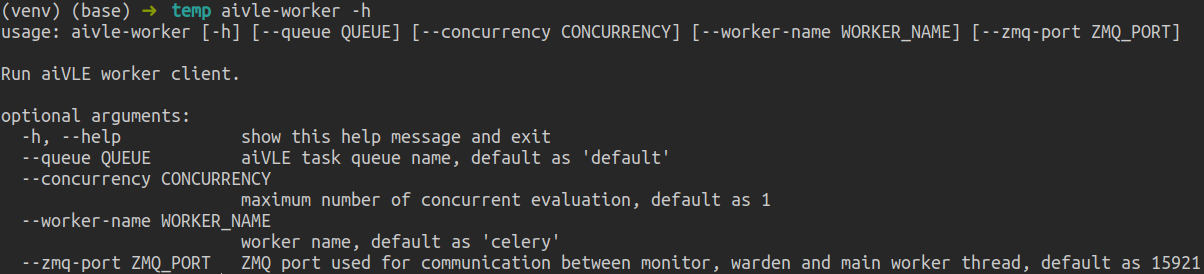
\includegraphics[width=\textwidth]{images/aivle-worker-cli.png}
    \caption{aiVLE Worker Command-line Interface}
    \label{fig:aivle-worker-cli}
\end{figure}

\subsection{Design Goal}
\label{ss:aivle-worker-design-goal}
For security purposes, the implementation is expected to achieve:
\begin{enumerate}
    \item \textbf{File access restriction}: agent program should have no access to directories that may contain sensitive data (e.g., private keys), and should have read only access to files necessary for its execution (e.g., Python binary, dependencies, agent, and environment source code).
    \item \textbf{Network restriction}: agent program should have no access to the Internet. Otherwise, (1) it may benefit from extra computation resources; (2) it may send out confidential runtime details (e.g., configuration of simulation environment) that allow users to fine-tune their program; both of which make the competition unfair.
    \item \textbf{Resource limit}: agent program should be terminated and reported if it exceeds RAM, VRAM or time limit.
\end{enumerate}

For scalability, in addition to the task queue system that manages all worker nodes and distributes evaluation jobs fairly and efficiently to the workers (see Section~\ref{ch:aivle-web_highly-available-task-queue}), on the worker side, a client that requires little permission and setup would be extremely helpful. It benefits horizontal scalability because 1) adding new worker nodes is easier, 2) more machines can be used as worker nodes (e.g., shared GPU servers, programming lab PCs). Thus, what we expect from this solution are:
\begin{enumerate}
    \item \textbf{Managed concurrency}: it should be able to run as many evaluation jobs concurrently as the hardware resource permits, while being able to detect and terminate processes that consume excessive RAM/VRAM. For more details please refer to Section~\ref{ss:aivle-worker-resource-awareness}.
    \item \textbf{Minimal permission requirement}: if we have access to run the submission locally, the environment should be able to operate as a worker node (i.e., sudo is not required).
    \item \textbf{Minimal dependency requirement}: any Linux machine with kernel version $\ge 5.4$ and Python version $\ge 3.8$ should be able to run the worker client.
    \item \textbf{Moderate overhead}: compared to traditional OJ, aiVLE can trade some overhead (both startup and runtime) for absolute essentials like GPU support. However, to achieve a certain level of throughput, warmup time as long as several minutes is still unacceptable.
\end{enumerate}

\subsection{Security Solution}
There are three mainstream security solutions for our consideration: 1) virtual machine (VM) such as Virtualbox, 2) container such as Docker/Podman, and 3) sandbox such as Firejail. The primary areas of interest are compared in Table~\ref{tab:security-solutions}\footnote{There are some caveats to the claims listed in this table. For more details please refer to Appendix~\ref{as:comparison-of-security-solutions}.}:

\begin{table}[H]
\centering
\begin{tabular}{|c|c|cc|c|}
\hline
\multirow{2}{*}{} & \textbf{VM} & \multicolumn{2}{c|}{\textbf{Container}} & \textbf{Sandbox} \\ \cline{2-5} 
 & VirtualBox & \multicolumn{1}{c|}{Docker} & Podman & Firejail \\ \hline
\textbf{Rootless} & No & \multicolumn{1}{c|}{Yes} & Yes & Yes \\ \hline
\textbf{Level of isolation} & Very high & \multicolumn{2}{c|}{High} & Medium \\ \hline
\textbf{Overhead} & High & \multicolumn{2}{c|}{Low} & None \\ \hline
\textbf{Startup time} & $\sim$15s & \multicolumn{2}{c|}{$\sim$3s} & $\sim$0.05s \\ \hline
\textbf{GPU support} & No & \multicolumn{2}{c|}{Yes, with NVIDIA container runtime} & Yes \\ \hline
\end{tabular}
\caption{Comparison of Mainstream Security Solutions}
\label{tab:security-solutions}
\end{table}

There are several must-haves for the candidate solution:

\begin{enumerate}
    \item GPU-support. Many recent RL algorithms are practically impossible to run without a GPU. This eliminates VM without PCI passthrough.
    \item Server needs to be shared. This eliminates VM with PCI passthrough as it requires exclusive access. This also eliminates Podman and Docker, as they prevent the GPU from being shared by any other container with root access.
\end{enumerate}

Therefore, Firejail is the only option left. I built a custom security profile to expose only the necessary file system and devices to processes inside the sandbox. I also used Firejail to impose CPU affinity (i.e., core count) and RAM usage limit on each sandbox.

\subsection{Resource Awareness}
\label{ss:aivle-worker-resource-awareness}
The architecture of aiVLE Worker's resource awareness is illustrated in Figure~\ref{fig:aivle-worker-resource-awareness-arch}. In the following subsections, we will discuss the objectives and design of related components, namely \texttt{monitor} and \texttt{warden} modules.

\begin{figure}[H]
    \centering
    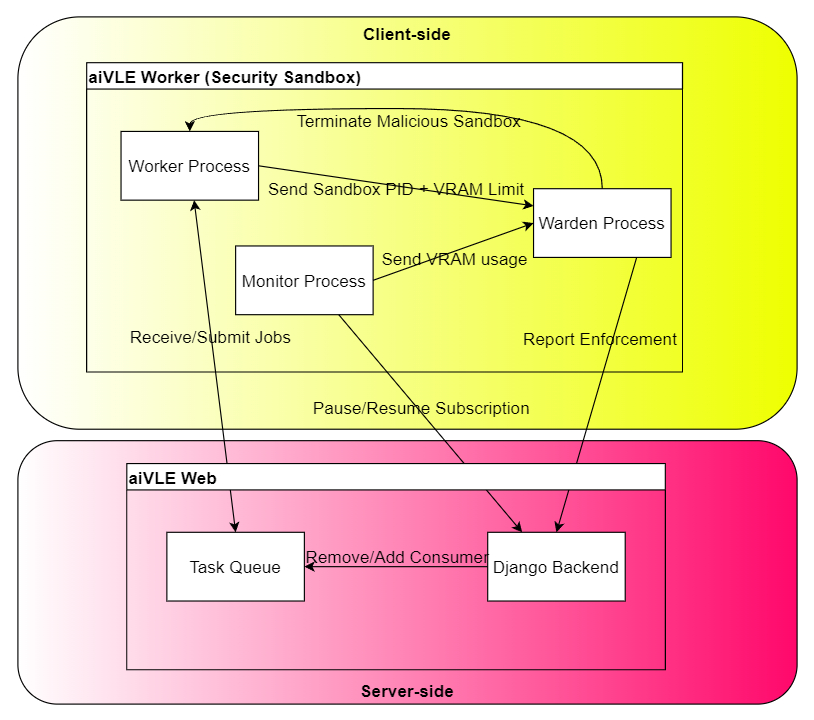
\includegraphics[width=0.8\textwidth]{images/aivle-worker-resource-awareness-arch.png}
    \caption{aiVLE Worker Resource Awareness Architecture}
    \label{fig:aivle-worker-resource-awareness-arch}
\end{figure}

\subsubsection{Resource Monitoring - \texttt{monitor} module}
\label{sss:monitor}
To achieve resource-sensitive load balancing, and to enforce resource limit, we need to monitor CPU/GPU utilization and RAM/VRAM usage and take actions accordingly. Therefore we implement the \texttt{monitor} module inside aiVLE Worker that runs in parallel with the main worker process. The \texttt{monitor} module:
\begin{enumerate}
    \item Monitors the system utilization periodically
    \item Controls the worker's task queue subscription according to prefetched threshold
    \item Sends monitoring metrics to the \texttt{warden} module to enable resource limit enforcement
\end{enumerate}

The first objective is achieved by the execution flow illustrated in Figure~\ref{fig:aivle-worker-monitor-flow} with the help of \href{https://pypi.org/project/psutil/}{\texttt{psutil}}\footnote{\href{https://pypi.org/project/psutil/}{https://pypi.org/project/psutil/}} for CPU/RAM monitoring and \href{https://github.com/fbcotter/py3nvml}{\texttt{py3nvml}}\footnote{\href{https://github.com/fbcotter/py3nvml}{https://github.com/fbcotter/py3nvml}} for GPU monitoring. The last objective involves inter-process communication that will be discussed later in detail with Figure~\ref{fig:aivle-worker-ipc}.

\begin{figure}[H]
    \centering
    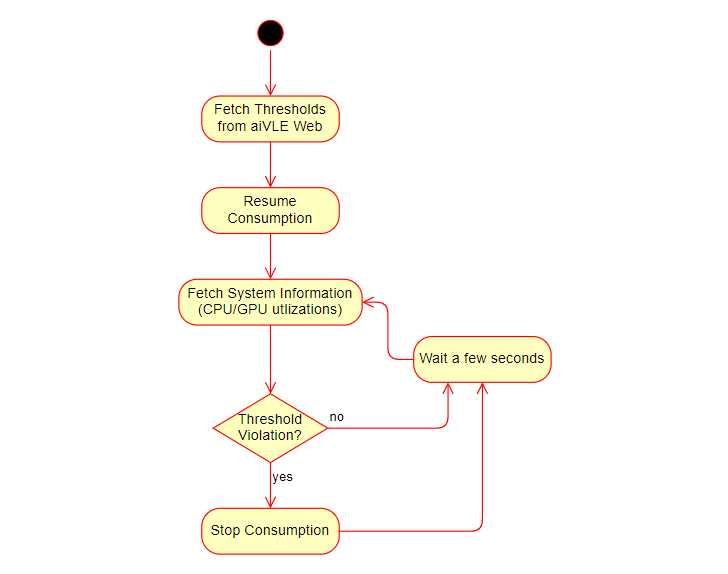
\includegraphics[width=0.45\textwidth]{images/aivle-worker-monitor-flow.png}
    \caption{Execution Flow of \texttt{monitor} module}
    \label{fig:aivle-worker-monitor-flow}
\end{figure}

Now we explain why the \texttt{monitor} module is also responsible for controlling the task queue subscription: Celery does not allow the worker itself to pause \textbf{consuming} tasks - the worker can only \textbf{shutdown} itself entirely, and only the master server can pause \textbf{sending} tasks to a certain worker. So we have two possible designs: either sending monitoring metrics periodically to the master server and let the master server have full control, or make the workers fetch the threshold on startup and request the master server to pause whenever the threshold is violated. The second option is our choice because it incurs much less communication overhead and a fixed, prefetch threshold works fine in our use case.

\subsubsection{Limit Enforcement - \texttt{warden} module}
\label{sss:warden}
The \texttt{warden} module is responsible for:
\begin{enumerate}
    \item Collecting task information from \texttt{worker} module
    \item Collecting system resource information from \texttt{monitor} module
    \item Terminating sandboxes that violates resource restrictions and report to aiVLE Web\footnote{We use ``master server'' and aiVLE Web interchangeably in the context of task queue because they run in the same Python monolithic server application.}
\end{enumerate}

Terminating sandboxes and reporting to aiVLE Web is straightforward - killing the corresponding PID and making an HTTP request. What makes \texttt{warden}'s job challenging is its first two objectives: there are three modules that run in parallel: \texttt{worker}, \texttt{monitor} and \texttt{warden}; they need to exchange information in order to collaborate. This is where ZeroMQ~\parencite{zeromq} comes handy: only the worker knows the mapping from sandbox PID to task information (i.e., VRAM limit), and only the \texttt{monitor} knows the VRAM usage of each process. Both need to send their data to the \texttt{warden} process which oversees all running jobs and terminates jobs that violate restrictions. Figure~\ref{fig:aivle-worker-ipc} shows the inter-process communication among these three:

\begin{figure}[H]
    \centering
    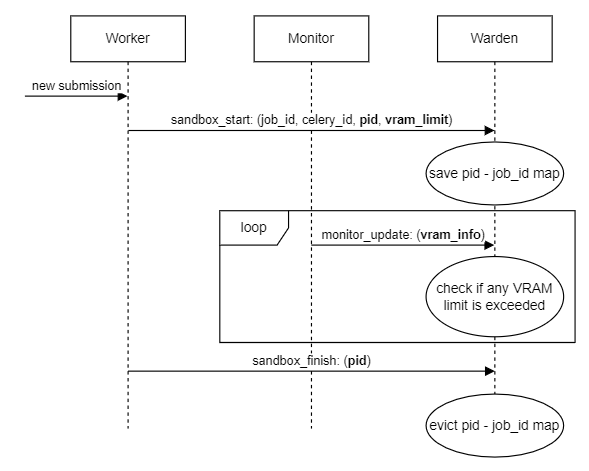
\includegraphics[width=0.8\textwidth]{images/aivle-worker-ipc.png}
    \caption{aiVLE Worker Inter-process Communication}
    \label{fig:aivle-worker-ipc}
\end{figure}

For \texttt{warden}'s case, every time it receives an update from \texttt{monitor}, it goes through the list of active sandboxes, queries the process hierarchy\footnote{This is necessary as most frameworks like PyTorch will spawn new processes for computation. Generally the process that is directly utilizing GPU is no longer the parent process. And there might be multiple processes in the same sandbox that consumes VRAM. By traversing the process tree recursively, we prevent intentional or unintentional attempts of ``downplaying'' the resource consumption of certain sandboxes.} to calculate the total VRAM usage of each sandbox, and finally checks if any sandbox needs to be terminated.

\section{aiVLE Web - AI Competition Platform}
\label{ch:aivle-web}
aiVLE Web consists of a Django backend that is $\sim$2.5K LoC and a React frontend that is $\sim$2K LoC. An active instance is deployed on the server and is accessible from \href{https://aivle.leotan.cn/}{https://aivle.leotan.cn/} (frontend) and \href{https://aivle-api.leotan.cn/}{https://aivle-api.leotan.cn/} (API and admin panel). Figure~\ref{fig:aivle-web-frontend-screenshot} shows a few screenshots of the React frontend. Note that we used mobile-sized screenshots due to limited space, but the design is responsive (i.e., it adapts to different screen sizes).

\begin{figure}[H]
    \centering
    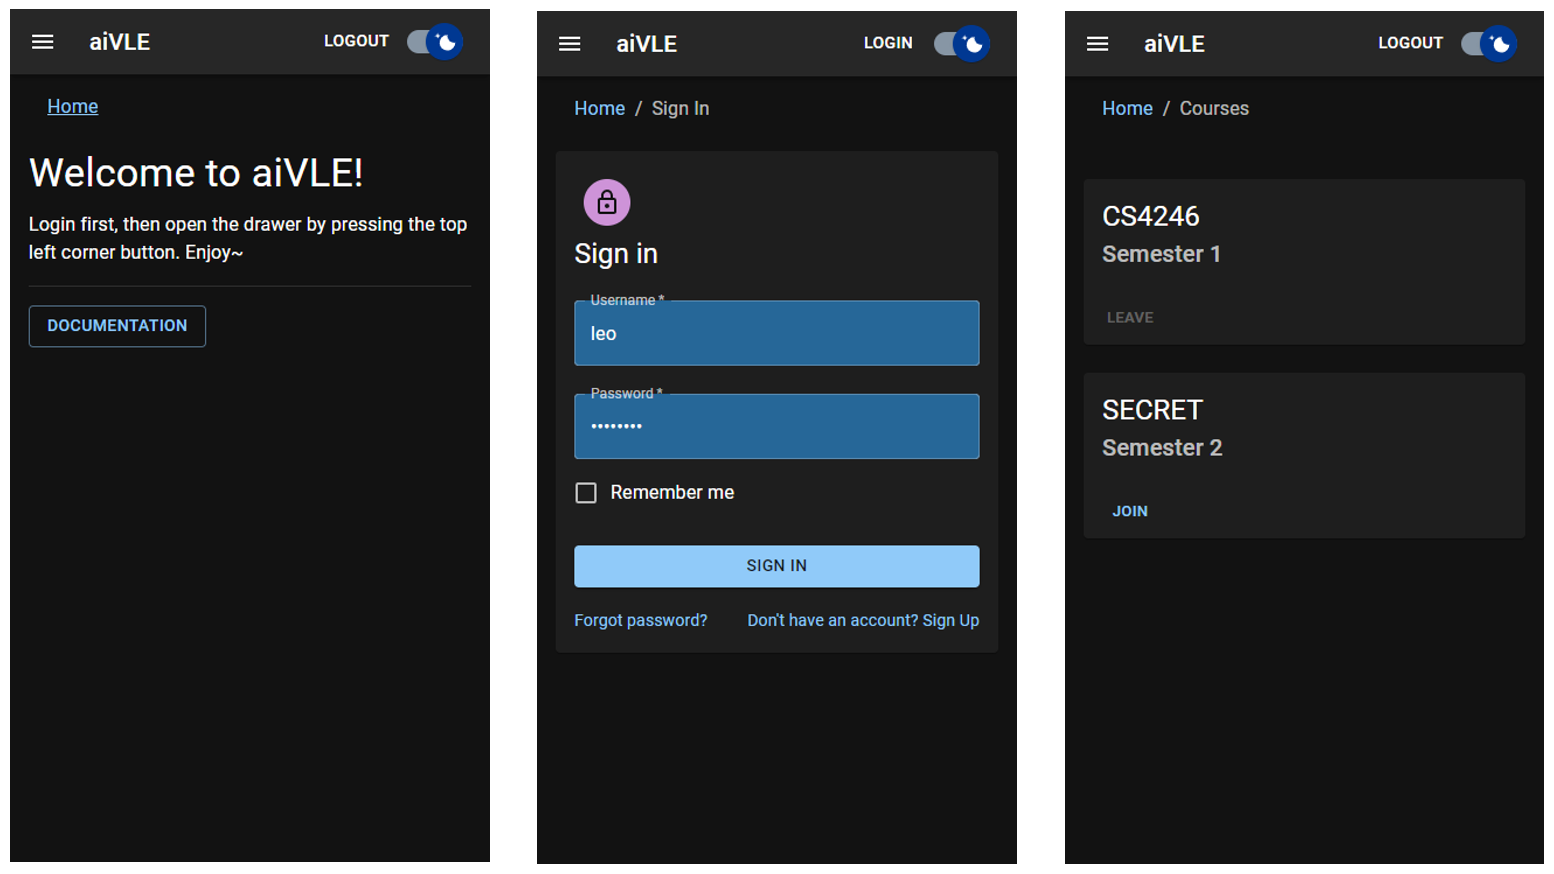
\includegraphics[width=\textwidth]{images/aivle-web-frontend-screenshot.png}
    \caption{aiVLE Web Frontend Screenshots}
    \label{fig:aivle-web-frontend-screenshot}
\end{figure}

\subsection{Design Goal}
There are three primary considerations to the design of aiVLE web: extensibility, scalability, and usability. 

\textbf{Extensibility} means the architecture should be extensible for future upgrades. One of the most significant architectural changes is the frontend-backend separation. This allows sophisticated data processing without making the backend codebase and API bloated - we will discuss one such scenario (course administration) in Section~\ref{ss:aivle-cli} for a tool named aiVLE CLI. In addition, to demonstrate the extensibility of our database model, we prepared a proposal on how to extend the existing codebase to support multi-agent competition (see Appendix~\ref{appendix:aivle-web_matchmaking}).

\textbf{Scalability} means the platform should be able to spread the evaluation workload, the most computationally heavy task, over many worker machines. We will discuss this objective in detail with 1) highly available and fault tolerant task queue (Section~\ref{ch:aivle-web_highly-available-task-queue}) and 2) resource-sensitive load balancing (Section~\ref{ss:aivle-web-load-balancing}).

\textbf{Usability} means the platform should provide all the features the users (e.g., CS4246 teaching team) need for a successful semester of teaching. While there are many features we could discuss, also due to space limit, we pick the role-based permission model (Section~\ref{ss:aivle-web-permission-model}) as a typical example of how we carefully balance complexity and flexibility during the development process.

\subsection{Highly Available and Fault Tolerant Task Queue}
\label{ch:aivle-web_highly-available-task-queue}
This is a continuation of \hyperref[ss:aivle-worker-design-goal]{scalability of (grading) workers}. In the section for aiVLE worker, we addressed the problem of running the worker on as many computers as possible with as little configuration/permission as possible. Here we address the problem of 1) coordinating the communication between the workers and the backend server, and 2) distributing grading tasks to the workers efficiently for shorter waiting time and higher resource utilization.
\subsubsection{The Problem}
In aiVLE 1.0, there was no concept of ``task queue''. All pending tasks are stored in the DB with the status ``QUEUED''. Communication between the worker (or runner as per the term used by original author) and server is \textit{half-duplex by polling}. In other words, the worker makes \textbf{periodic} requests to the server for new ungraded submissions:
\begin{figure}[H]
    \centering
    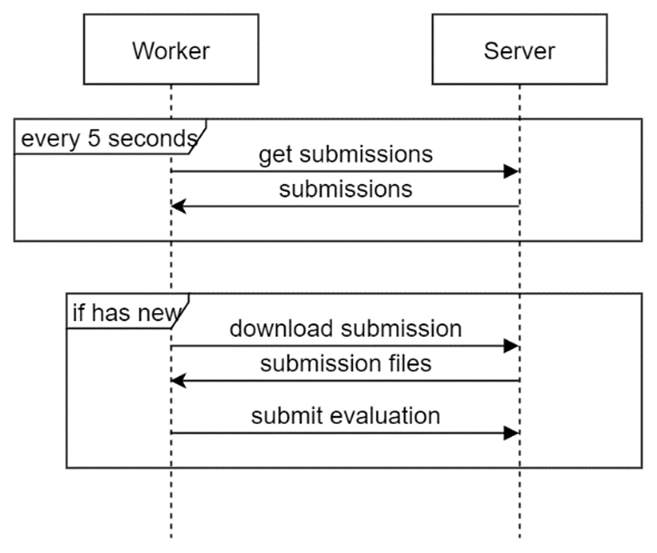
\includegraphics[width=0.5\textwidth]{images/aivle-web-old-task-queue.png}
    \caption{Old aiVLE “Task Queue”}
    \label{fig:aivle-web-old-task-queue}
\end{figure}
There are three critical limitations to this approach:
\begin{enumerate}
    \item Worker-side polling does not scale well: there is no mechanism in orchestrating the timing and order of workers polling the server for new jobs. The severity of possible traffic spike (i.e., many workers poll the server at the same time due to lack of coordination) increases linearly with the number of worker nodes.
    \item Race condition: if two worker pull submissions at the same time, both will get the same ungraded submission. Such redundant work will get more significant with more worker nodes, which hurts the overall efficiency of the worker cluster.
    \item No concurrency in each worker\footnote{In the actual use of aiVLE 1.0, we run multiple worker clients on the same machine for disguised concurrency. Besides the inconvenience of manually starting multiple worker clients, this approach makes managing resources difficult as each client runs without knowing the existence of others even if they are on the same machine.\label{fn:worker-disguised-concurrency}}: each individual worker only polls for new job when it has no submission to grade. In other words, each worker can only grade one submission at a time.
    \item No load balancing: the backend has no control over which worker grades which submission, therefore load balancing is virtually impossible
\end{enumerate}

\subsubsection{The Solution}
Similar to the idea of extracting the responsibility of data storage/management into a separate database backend, we delegate the messaging tasks to a message queue (MQ). Conceptually, message queue enables asynchronous communication between clients (who submit tasks) and workers (who finish tasks). As for implementing the concept in our Python web application, we used \href{https://docs.celeryq.dev/en/stable/}{Celery} framework with \href{https://www.rabbitmq.com/}{RabbitMQ} message queue broker/backend. Figure~\ref{fig:aivle-web-mq} illustrates how the MQ-based task queue works:

\begin{figure}[H]
    \centering
    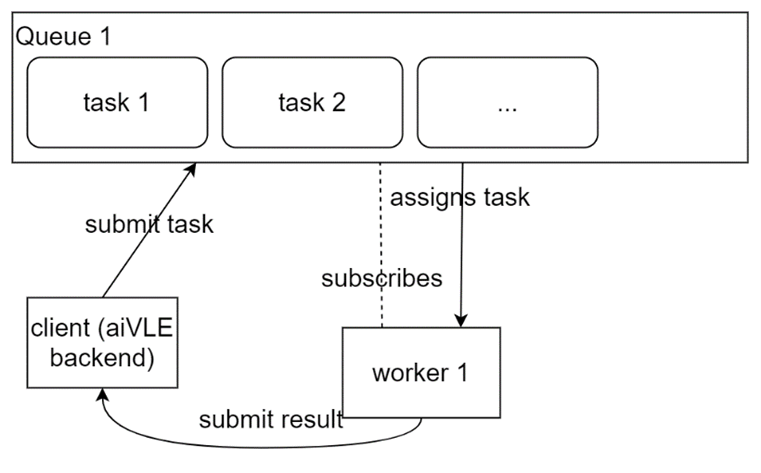
\includegraphics{images/aivle-web-mq.png}
    \caption{Message Queue Based Task Queue}
    \label{fig:aivle-web-mq}
\end{figure}

Every worker listens to one or more ``queues'', where the message broker is responsible for allocating tasks fairly among workers in each queue. When an evaluation job arrives, aiVLE backend will submit the job to an appropriate queue (i.e., private queue if user has dedicated workers available, otherwise public CPU/GPU queue according to task specification) and wait for the assigned worker to submit evaluation result. The task will remain in the queue until it is processed (i.e., message queue is persistent). A randomly generated task ID is used to authenticate worker's submission – only the worker whom the broker assigned the task to will have this ID. This approach not only reduces the number of requests to be $O(n)$ where $n$ is the number of evaluation jobs, but also ensures fair distribution of tasks among workers. Moreover, we also benefit from other standard features of message queue such as automatic retry and heartbeat checks.

\subsection{Resource-sensitive Load Balancing}
\label{ss:aivle-web-load-balancing}
By using message queue for task distribution, we already have some primitive load balancing - Celery with RabbitMQ backend\footnote{Celery is a Python task queue library. RabbitMQ is the default message queue broker for Celery.} by default dispatches messages to all consumers in round-robin style, therefore all consumers are expected to consume the same number of tasks from the same queue over a fixed period of time. Although this is a huge improvement over no load balancing at all, from some stress testing using real-world workload, we find it necessary to take system load into consideration. Specifically, the primitive method of load balancing by number of tasks works poorly when certain tasks are much more resource intensive. For example, assume both worker A and worker B receive 5 submissions, but the ones for worker A consumes 30\% of total VRAM while the ones for worker B takes only 10\% of total VRAM. There are two serious implications in this imaginary scenario:
\begin{enumerate}
    \item \textbf{Unfairness}: suppose the worker is configured to run at most 8 concurrent evaluations, the fourth and fifth submissions arriving at worker A will not have sufficient VRAM. They will likely receive runtime errors which are unacceptable.
    \item \textbf{Inefficiency}: suppose the task queue is configured to automatically retry the failed job by putting a new evaluation job into the same queue, since worker A is still accepting submissions, the retry attempt may take additional fails to finally arrive at worker B.
\end{enumerate}

The key to solving such unwanted behavior is 1) to monitor the available system resources, 2) to stop processing new tasks when the available resources fall below certain thresholds. Most heavy-lifting is handled on the worker side (see Section~\ref{ss:aivle-worker-resource-awareness}). As for aiVLE Web, it uses \texttt{add\_consumer} and \texttt{cancel\_consumer} Celery APIs for resuming and pausing consuming respectively. Nevertheless, there are two points to note in this solution:

\begin{enumerate}
    \item It does not cancel already running jobs. Instead, it only stops dispatching new tasks to the worker where the threshold is met. This behavior is acceptable in our case since we only need to promise submissions with a certain amount of resources to run the job, and our solution guarantees\footnote{Technically speaking, this guarantee does not hold between two checks on system information, but we can easily reduce the impact by performing the check more frequently. In our experience, one second interval is more than enough.} the promised amount of CPU/RAM/VRAM at the beginning of any evaluation job.
    \item It does not balance the resource utilization among all workers. \texttt{cancel\_consumer} simply removes the worker from the list of consumers to dispatch tasks to. To achieve resource utilization balance, aiVLE Web needs to understand each worker's utilization in real-time and dispatch tasks accordingly. We think the overhead (i.e., network traffic for reporting utilization data) and complexity (i.e., load balancing algorithm) of this design significantly outweighs the potential benefits.
\end{enumerate}

Besides addressing the previously mentioned implications, resource-sensitive load balancing greatly increases the system utilization. Without resource awareness, aiVLE 1.0 could only achieve disguised concurrency by running multiple worker clients on the same machine. To ensure the machines will not be overloaded, we could only ``play it safe'' by always under-utilizing the resources. For example, the current configuration of aiVLE 1.0 only allows 3 concurrent evaluations, resulting in an average of $\sim30\%$ of volatile GPU usage. In comparison, we can achieve up to 85\% GPU utilization rate, and with the later introduced resource-sensitive load balancing, overloading the system is no longer a concern. This translates to roughly three times\footnote{In real world use you might not want to set the threshold to be as high as 85\%, but even with a conservative 80\% threshold the improvement is still very significant.} of a performance improvement.

\subsection{Role-based Permission Model}
\label{ss:aivle-web-permission-model}
In Django we have two major types of permission model: per-model permission (built-in authentication system) and per-object permission (\href{https://github.com/django-guardian/django-guardian}{django-guardian}). Per-model permission means the finest granularity is model-level, that is we may only check if the user has read/write/edit/delete access to the model. Per-object permission is the finest granularity possible as we can establish arbitrary permission between any object and any user. In fact, the worst possible space complexity is $O(mnk)$ where $m$ is the number of objects, $n$ is the number of users and $k$ is the number of permissions.

In our use case, model-based permission is too coarse-grained: a student should only be able to view the tasks in the course he/she enrolled in, rather than all the tasks available on the platform. On the other hand, object-based permission is overkill: there might be hundreds of thousands of job records in the database, storing each user's permission to each job record is simply too wasteful. Therefore, we propose a solution that is the sweet spot between the two extremes: role-based permission model.

The entity relationship diagram of aiVLE Web is illustrated in Figure~\ref{fig:aivle-web-er-diagram}:
\begin{figure}[H]
    \centering
    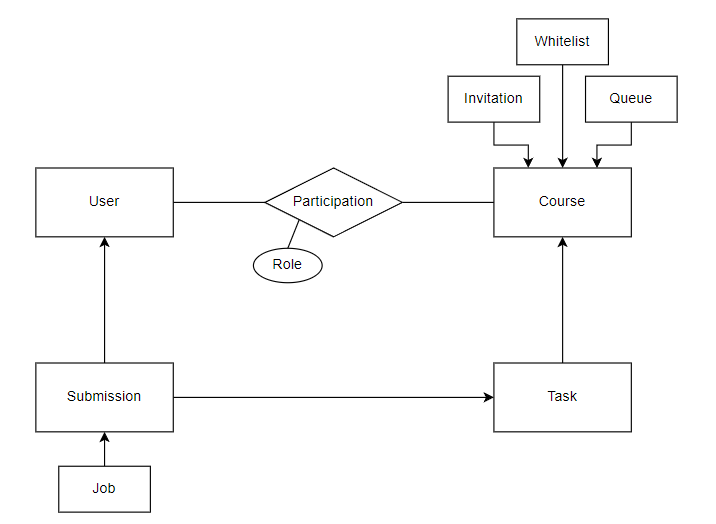
\includegraphics[width=0.8\textwidth]{images/aivle-web-er-diagram.png}
    \caption{aiVLE Web Entity Relationship Diagram}
    \label{fig:aivle-web-er-diagram}
\end{figure}

In the relational entity Participation, we record the ``role'' of the User in a Course. Possible roles\footnote{Note that a user can have different roles in different courses. And superuser who has access to absolutely everything is not in the scope of this discussion.} (as defined in \texttt{app.model.participation}) are: administrator (ADM), lecturer (LEC), teaching assistant (TA), student (STU) and guest (GUE).

The idea of role-based permission model is centered around one's role in the corresponding course: to determine one's access to any object, we first find the object's related course, then check if the user has access to this object in the context of this related course. For example, if we need to know if the user has view access to a certain \texttt{Job}, we can follow the arrows in the diagram: Job $\to$ Submission $\to$ Task $\to$ Course $\to$ Participation $\to$ User to find the corresponding role\footnote{The utility function \texttt{has\_perm} automatically queries the role given the course and the user, so its argument is the course instead of the role.}, and check if this role has \texttt{job.view} permission according to the permission lookup table (see Table~\ref{tab:aivle-web-permission-table}).

By introducing the \texttt{Participation} relational entity and \texttt{has\_perm(course, user, permission)} utility function, we compressed the worst case $O(mnk)$ space complexity to $O(nk)$ and it is a significant improvement. In reality the number of objects $m$ significantly outweighs the number of users $n$ or permissions $k$. We can summarize different roles' access (as defined in aiVLE.settings.ROLES) using a permission matrix in Table~\ref{tab:aivle-web-permission-table}:

\begin{table}[H]
\centering
\begin{tabular}{|c|l|l|l|l|l|l|}
\hline
\multicolumn{1}{|l|}{} &  & Admin & Lecturer & TA & Student & Guest \\ \hline
\multirow{5}{*}{Task} & View opened tasks & x & x & x & x & x \\ \cline{2-7} 
 & View all tasks & x & x & x &  &  \\ \cline{2-7} 
 & Add task & x & x &  &  &  \\ \cline{2-7} 
 & Edit task & x & x & x &  &  \\ \cline{2-7} 
 & Delete task & x & x &  &  &  \\ \hline
\multirow{4}{*}{Submission} & View own submissions & x & x & x & x &  \\ \cline{2-7} 
 & View all submissions & x & x & x &  &  \\ \cline{2-7} 
 & Add submission (under own name) & x & x & x & x &  \\ \cline{2-7} 
 & Download submission & x & x &  &  &  \\ \hline
\end{tabular}
\caption{Partial Permission Lookup Table}
\label{tab:aivle-web-permission-table}
\end{table}

\subsection{aiVLE CLI - Course Administration Utility}
\label{ss:aivle-cli}

aiVLE CLI is an interactive command-line tool written in ($\sim$ 500 lines of) Go. It is cross-compiled\footnote{Cross-compilation means using platform A to build a binary that runs on platform B.} to native binary on Windows, Linux and macOS (Intel + Apple Silicon) so that the facilitators can enjoy the same convenience on any platform they prefer. Users make use of this program by answering questions and selecting choices as shown in Figure~\ref{fig:aivle-cli}.

\begin{figure}[H]
    \centering
    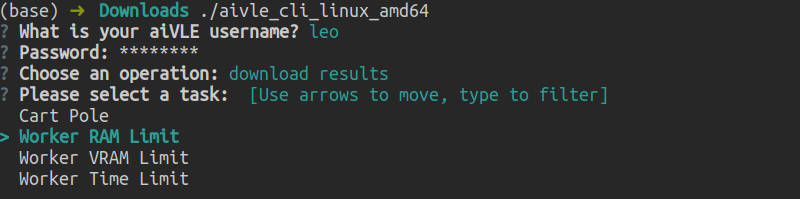
\includegraphics[width=\textwidth]{images/aivle-cli.png}
    \caption{aiVLE CLI Usage}
    \label{fig:aivle-cli}
\end{figure}

There are two reasons behind building a separate application for course administration on the client side instead of integrating all these functionalities into aiVLE Web. First, it is easier to develop a command-line program compared with both a backend API (logic) and corresponding web frontend (user interface). For a command-line app, work required for the user interface is negligible and we only need to focus on delivering the logic. Second, KISS (keep it simple, stupid) principle. Ideally, if a complex functionality can be implemented with several smaller yet more general operations without significant performance or usability penalty, we should avoid providing such a complex API and let the caller do the composition. Note that such composition is impossible without frontend-backend separation, since before the separation the only way of interacting with the data is to use the website, and the website itself, while friendly to us humans, is not as useful as raw data to computer programs.

Currently the aiVLE CLI has 4 features:

\begin{enumerate}
    \item Download submissions: given a task, you may download all submissions (evaluation result included) or only those are marked for grading.
    \item Download evaluation results: given a task, you may download a CSV file with username, grade, and evaluation details.
    \item Upload student emails to the course whitelist: the utility can parse and upload student roster Excel file exported from LumiNUS.
    \item Get API token from username and password.
\end{enumerate}
\chapter{Deployment and Testing}
\label{ch:deployment-and-testing}
aiVLE 2.0, especially aiVLE Worker and aiVLE Grader, is designed to be highly scalable and easy to deploy. However, just like any distributed systems, being able to run the individual components on a single machine is one thing, having all the components cooperate on separate machines to achieve actual distribution is another. Thus, to pave way for production deployment in the next academic year, and to demonstrate the actual performance of such a distributed system, we performed a complete deployment using several SoC cluster nodes and did several experiments/benchmarks on the system.

There are three sections covering both the deployment and tests this chapter: Section~\ref{s:deployment} describes the deployment environment and deployment steps. Section~\ref{s:load-balance-exp} discusses the experiment of load balancing among \textbf{multiple} worker nodes. Section~\ref{s:concurrency-exp} discusses the experiment of running evaluation jobs concurrently on a \textbf{single} worker node.

\section{Deployment}
\label{s:deployment}
Note that this deployment happened during the winter break (November 2021 to January 2022). Therefore some later updates to the aiVLE Web and Worker were not included during this deployment (most notably, resource-sensitive load balancing as mentioned in Section~\ref{ss:aivle-worker-resource-awareness} and Section~\ref{ss:aivle-web-load-balancing}). However, this does not affect the test results as the experiments are designed to have no system overloading (more on that later).

In specific, the exact versions used are (tag with GitHub link):
\begin{itemize}
    \item aiVLE Web: deploy-1 (\href{https://github.com/edu-ai/aivle-web/releases/tag/deploy-1}{https://github.com/edu-ai/aivle-web/releases/tag/deploy-1})
    \item aiVLE Worker: v0.1.2 (\href{https://github.com/edu-ai/aivle-worker/releases/tag/v0.1.2}{https://github.com/edu-ai/aivle-worker/releases/tag/v0.1.2})
\end{itemize}

\subsection{Environment}
\label{ss:deployment-environment}
aiVLE Worker is deployed on SoC compute cluster \texttt{xgpg0, xgpg1, xgpg2} with the following configuration:
\begin{itemize}
    \item Operating System (Code~\ref{code:deployment-os}): Ubuntu 20.04 LTS with Linux kernel version 5.4.0
    \item GPU (Code~\ref{code:deployment-gpu}): NVIDIA A100-PCI, Driver 495.29, CUDA 11.5
    \item CPU: 2x AMD Epyc 7352, in total 48 cores/96 threads, base clock 2.3GHz
    \item RAM: 256GiB DDR4
\end{itemize}

\begin{code}
\begin{minted}[frame=lines,framesep=2mm,baselinestretch=1.2,bgcolor=LightGray,fontsize=\footnotesize,linenos,samepage]{shell}
> cat /proc/version
Linux version 5.4.0-91-generic (buildd@lcy01-amd64-017) 
(gcc version 9.3.0 (Ubuntu 9.3.0-17ubuntu1~20.04)) #102-Ubuntu SMP Fri Nov 5 16:31:28 UTC 2021
\end{minted}
\captionof{listing}{Deployment Environment - Operating System}
\label{code:deployment-os}
\end{code}

\begin{code}
\begin{minted}[frame=lines,framesep=2mm,baselinestretch=1.2,bgcolor=LightGray,fontsize=\footnotesize,linenos,samepage]{shell}
> nvidia-smi
+-----------------------------------------------------------------------------+
| NVIDIA-SMI 495.29.05    Driver Version: 495.29.05    CUDA Version: 11.5     |
|-------------------------------+----------------------+----------------------+
| GPU  Name        Persistence-M| Bus-Id        Disp.A | Volatile Uncorr. ECC |
| Fan  Temp  Perf  Pwr:Usage/Cap|         Memory-Usage | GPU-Util  Compute M. |
|                               |                      |               MIG M. |
|===============================+======================+======================|
|   0  NVIDIA A100-PCI...  On   | 00000000:01:00.0 Off |                    0 |
| N/A   49C    P0    36W / 250W |      0MiB / 40536MiB |      0%      Default |
|                               |                      |             Disabled |
+-------------------------------+----------------------+----------------------+
\end{minted}
\captionof{listing}{Deployment Environment - GPU}
\label{code:deployment-gpu}
\end{code}

aiVLE Web is deployed on a \href{https://linode.com/}{Linode} Nanode 1GB VPS (virtual private server) with 1 virtual CPU core and 1 GiB of RAM. We carefully picked the parameters to avoid the aiVLE Web server being the bottleneck of all experiments (see Section~\ref{sss:choice-of-params}).

\subsection{Limitations}
\label{ss:deployment-limitations}
As with every distributed system, even if the system works on a few machines, it does not necessarily mean the system will work or scale well to dozens or even hundreds of machines. While we design the system to be highly scalable, and the underlying technologies (i.e., Celery as Python library and RabbitMQ as message queue broker) have proven to be effective on hundreds of machines, we are never certain until we actually scale the system to that many nodes and put it under pressure.

Unfortunately, for the time being, we are unable to materialize such a large-scale experiment: as we could only secure access to three machines in the SoC compute cluster. Also, at the moment, the tasks were not demanding enough to put the system at such a scale under considerable pressure. For example, on the \texttt{xgpg*} nodes used for this experiment, every evaluation takes $\sim$10 seconds to finish, which is too short for even tens of worker nodes. For the evaluation subsystem to be stressed, we at least need to keep the task queue ``filled''. In other words, the rate of submitting new jobs into the task queue should be comparable to the rate of workers finishing jobs. However, with each job only taking $\sim$10 seconds, suppose we have 50 workers, our rate of consumption would be $50/10=5$ jobs per second (every 10 seconds we can process 50 jobs). If we assume each submission to be $\sim$20MiB\footnote{Many deep learning models are much larger, so we are having a relatively conservative estimation here.}, it would require at least 100MiB per second of network throughput, which is already approaching the limit of gigabit Ethernet available on most machines.

Therefore, with our current resources and setup, we could not properly evaluate the scalability potential of aiVLE 2.0. However, our experiment setup is on par with the resources available to the CS4246 teaching team, and aiVLE 2.0 is shown to have a much higher utilization rate of computational power. As a result, aiVLE 2.0 can process submissions with much smaller delays. In addition, properties like fair distribution and small worker overhead remain stable regardless of the number of nodes, so they were properly evaluated in our experiments.

To summarize, we are cautiously optimistic about the scalability of aiVLE 2.0 as we do not yet have experiment data to support it, but we are confident that it can support CS4246 teaching much more effectively from the results.

\subsection{Steps}
To simulate the production deployment process, we started everything afresh. The following steps\footnote{Detailed deployment guide with common Q\&A on the documentation website: \href{https://edu-ai.github.io/aivle-docs/dev-guide/deployment-guide/}{https://edu-ai.github.io/aivle-docs/dev-guide/deployment-guide/}} are sufficient for any deployment from the ground up:

\begin{enumerate}
    \item Prepare the message queue broker: either by installing \href{https://www.rabbitmq.com/}{RabbitMQ} or using cloud message queue provider such as \href{https://www.cloudamqp.com/}{CloudAMQP}. In our case, we installed RabbitMQ on the same VPS with aiVLE Web.
    \item Install and start aiVLE Web on the master server.  The aiVLE Web Read-me\footnote{\href{https://github.com/edu-ai/aivle-web\#readme}{https://github.com/edu-ai/aivle-web\#readme}} is the definitive guide on this process.
    \item Setup the users, courses, tasks in aiVLE Web via its RESTful API or Django admin panel.
    \item Prepare the worker nodes with necessary dependencies (i.e., Firejail, Pip, Virtualenv, CUDA drivers). In our case, we requested the cluster admins to install Firejail as all other dependencies are already available.
    \item Install and start aiVLE Worker on the worker nodes. aiVLE Worker Read-me\footnote{\href{https://github.com/edu-ai/aivle-worker\#readme}{https://github.com/edu-ai/aivle-worker\#readme}} describes this process in detail.
\end{enumerate}

There are some issues we found during the deployment process. None of which is critical in a sense that we eventually found workarounds without modifying any existing codebase or design. You may find the details in Appendix~\ref{appendix:deployment-issues}.

\section{Load Balance Experiment}
\label{s:load-balance-exp}
In this section, we will discuss the experiments about load balancing evaluation jobs among \textbf{multiple} worker nodes. There are three objectives for this series of experiments:

\begin{enumerate}
    \item Show that the evaluation system scales well horizontally to several worker nodes.
    \item Show that the tasks are distributed evenly among worker nodes.
    \item Show that the worker nodes are fully utilized during stressful load.
\end{enumerate}

Raw logs and analyzing scripts can be found in \href{https://github.com/edu-ai/aivle-experiment-logs}{aiVLE experiment logs repository}\footnote{\href{https://github.com/edu-ai/aivle-experiment-logs}{https://github.com/edu-ai/aivle-experiment-logs}}. Correspondence between experiment setup and log file index is shown in Table~\ref{tab:load-balance-exp}.

\begin{table}[H]
\centering
\begin{tabular}{|c|c|c|c|c|c|}
\hline
\multicolumn{1}{|l|}{\begin{tabular}[c]{@{}l@{}}Web\\ log index\end{tabular}} & \multicolumn{1}{l|}{\begin{tabular}[c]{@{}l@{}}Worker\\ log index\end{tabular}} & \multicolumn{1}{l|}{Node count} & \multicolumn{1}{l|}{\begin{tabular}[c]{@{}l@{}}Concurrency \\ of worker\end{tabular}} & \multicolumn{1}{l|}{Submission count} & \multicolumn{1}{l|}{\begin{tabular}[c]{@{}l@{}}Concurrency \\ of submission\end{tabular}} \\ \hline
5 & 2 & 3 & 8 & 100 & 100 \\ \hline
6 & 3 & 2 & 8 & 100 & 100 \\ \hline
7 & 4 & 1 & 8 & 100 & 100 \\ \hline
\end{tabular}
\caption{Load Balancing Experiment Setup}
\label{tab:load-balance-exp}
\end{table}

\subsection{Methodology}
\label{ss:lb-exp-meth}
Since the evaluation task and all worker nodes are exactly the same, we have four parameters/variables to adjust:
\begin{enumerate}
    \item Node count: number of active nodes during the experiment.
    \item Concurrency of worker: maximum number of concurrent evaluation jobs allowed on \emph{each} worker node.
    \item Submission count: number of evaluation jobs submitted to the task queue.
    \item Concurrency of submission: maximum number of threads submitting jobs concurrently. Note that if this number is comparable to the submission count, master server will be blocked until all submissions are accepted (i.e., it will not distribute evaluation jobs to any of the worker nodes until all submissions are well-received)\footnote{This is because the submission rate is significantly larger than how fast the master server can process requests, and these submissions will pile up in the requests queue. Since the master server processes requests on a first-come, first-served basis, it is effectively blocked before all submissions are accepted. Of course this number cannot grow indefinitely as any machine will eventually run out of available threads or network bandwidth. Consequently, the submission count cannot grow indefinitely either as it should be comparable to the concurrency of submission. Section~\ref{sss:choice-of-params} will discuss the preliminary experiments that aim to find these upper bounds.\label{fn:concurrency-of-submission}}.
\end{enumerate}

In this section and Section~\ref{s:concurrency-exp}, submission count and concurrency of submission are both 100. This means before the first job is assigned to any of the worker nodes, 100 jobs are already queued. This is to ensure there will always be sufficient tasks for the workers to work on - if concurrency of submission is significantly smaller than the number of submissions, then the rate of submitting job may dictate the rate of workers finishing jobs, which is undesirable for our stress-oriented experiments.

For load balance experiment, we \textbf{fix concurrency on all workers to be 8}, measure \textbf{time taken} to finish 100 submissions with
\begin{itemize}
    \item 1 node (\texttt{xgpg0})
    \item 2 nodes (\texttt{xgpg0,1})
    \item 3 nodes (\texttt{xgpg0,1,2})
\end{itemize}

On the master server (aiVLE Web), we logged the critical phases of each submission with a timestamp, in specific, there is a timestamped record when
\begin{enumerate}
    \item submission is received
    \item evaluation job is submitted to task queue
    \item evaluation job is picked up by a worker
    \item evaluation job is being worked on by a worker
    \item evaluation job is terminated (either finished or failed)
\end{enumerate}

The start time is defined to be the earlier of 1) the latest ``submission is received'' record or 2) the earliest ``evaluation job is picked up by a worker'' record. The finish time is defined to be the latest ``evaluation job is terminated'' record. The total time is defined to be the difference between the finish time and the start time. The detailed method of calculating time taken to finish all submissions can be found in the \href{https://github.com/edu-ai/aivle-experiment-logs/blob/main/web/analyze.ipynb}{analyze script}. Note that the focus of this experiment is on the \textbf{evaluation subsystem}, not the entire system. For example, before we can start evaluation jobs, we need to upload the student submission first. However, the upload itself could take a significant amount of time depending on the server workload. Such preparation time is an irrelevant variable and should be excluded from our calculation. The definition of the start time here, combined with our effort to adjust the parameters such that evaluation starts only after all submissions are received, achieved such exclusion.

On each worker node, we also logged the timestamped GPU utilization rate and VRAM usage periodically (Figure~\ref{fig:experiment-lb-utilization-plot}). This helps us understand whether all worker nodes are busy most of the time - unnecessary idling is a sign of poor load balancing.

\begin{figure}[H]
    \centering
    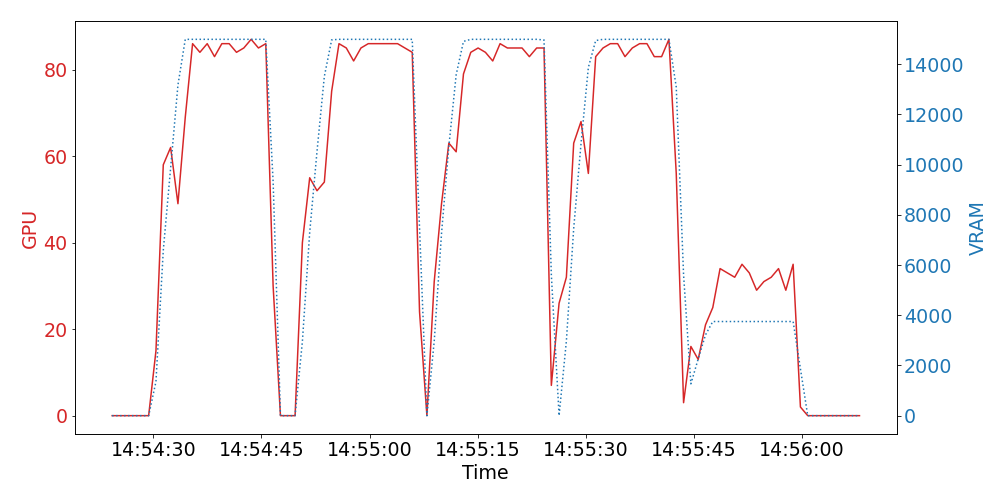
\includegraphics[width=\textwidth]{images/worker-utilization.png}
    \caption{GPU/VRAM Utilization Plot from \texttt{xgpg0\_2.log}}
    \label{fig:experiment-lb-utilization-plot}
\end{figure}

\subsubsection{Choice of Parameters}
\label{sss:choice-of-params}

There are two parameters that remain unexplained: number of total submissions (100) and maximum concurrent evaluations on each worker (8).

For the maximum concurrency allowed on each worker, we want the concurrency to be as large as possible (so that we properly ``stress'' the system) without overwhelming the system (so that the scaling overhead is mostly because of our task queue system instead of overwhelmed worker nodes). Since our evaluation task is mostly GPU-bounded, we performed experiments on a single machine with concurrent evaluation ranging from 2 to 16 and observed both the \textbf{GPU} utilization and \textbf{VRAM} utilization. However, with 40GiB of VRAM, it is hard to overload the VRAM even with 16 concurrent jobs as each job takes less than 2GiB of VRAM. On the other hand, GPU utilization increases linearly with number of concurrent jobs until more than 8 jobs. Increasing more jobs will not significantly increase the GPU utilization after 8 jobs, indicating that the machine could only handle up to 8 jobs without significantly degraded per-job performance.

For the total submission count, it is bounded by the maximum concurrent submission our server and network can handle. We performed preliminary experiments with 1500 (\href{https://github.com/edu-ai/aivle-experiment-logs/blob/main/web/debug.log.1}{\texttt{debug.log.1}}) and 250 (\href{https://github.com/edu-ai/aivle-experiment-logs/blob/main/web/debug.log.4}{\texttt{debug.log.4}}) total submissions, and found the submission client could not reach sufficient request concurrency (i.e., large enough such that no evaluation will happen before all submissions are received) in both cases. In fact, for \texttt{debug.log.1} and \texttt{debug.log.4}, the average time taken to finish evaluating one submission is $\sim$25 seconds, and we did observe evaluation jobs started before submissions are concluded. Given that the optimal time (i.e., time taken without any communication overhead) is $\sim$15 seconds, this confirms our intuition that not queuing up all submissions before starting evaluation severely hurts the accuracy of these experiments. On the contrary, for scenarios listed in Table~\ref{tab:load-balance-exp}, the average time is $\sim$18 seconds, which is much closer to the optimal time, and $\sim$3 seconds of overhead seems acceptable considering it needs to download and decompress the student submission first.

\subsection{Results}
\label{ss:load-balancing-exp-results}

First, for the performance of load balancing, below are the times for each test case:

\begin{itemize}
    \item 1 node: 235.426s (baseline)
    \item 2 nodes: 128.261s (91.78\%)
    \item 3 nodes: 92.475s (84.86\%)
\end{itemize}
The percentage is the scaling efficiency defined by $\frac{\text{Optional time}}{\text{Measured time}}\times 100\%$ where \emph{Optimal Time} is defined as $\frac{t_0}{N}$ where $N$ is the number of nodes and $t_0$ is the time taken with one node. We have observed satisfactory scaling efficiency in both 2-node and 3-node configurations.

Second, for the fairness of load balancing, below are the numbers of jobs assigned to each worker node (when there are more than one node):

\begin{itemize}
    \item 2 nodes: \texttt{\{celery@xgpg0: 50, celery@xgpg1: 50\}}
    \item 3 nodes: \texttt{\{celery@xgpg0: 34, celery@xgpg1: 36, 'celery@xgpg2': 30\}}
\end{itemize}
The jobs are nearly equally distributed in both cases, meaning that our round-robin load balancing mechanism is working as expected.

Third, for the utilization of system resources, since our task is GPU-bound, Figure~\ref{fig:experiment-lb-utilization-plot} plots the GPU and VRAM utilization for one of the worker nodes (others are similar). We have observed stable GPU utilization of $\sim 85\%$ at peak, and a busy rate of $\sim 96\%$, meaning we have very good utilization of worker node resources.

\begin{figure}[H]
    \centering
    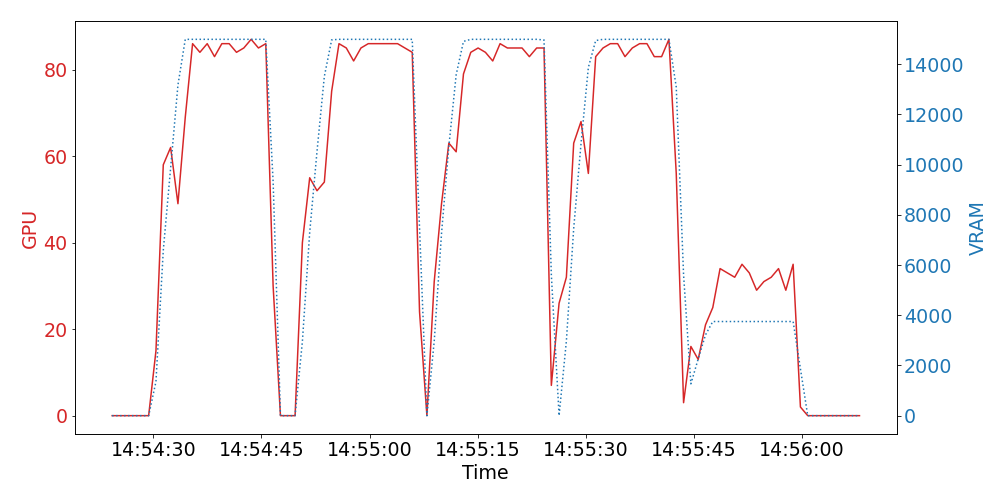
\includegraphics[width=\textwidth]{images/worker-utilization.png}
    \repeatcaption{fig:experiment-lb-utilization-plot}{GPU/VRAM Utilization Plot from \texttt{xgpg0\_2.log}}
\end{figure}

\section{Concurrency Experiment}
\label{s:concurrency-exp}
In this section, we will discuss the experiments about running multiple evaluation jobs \textbf{concurrently} on a \textbf{single} worker node. The objective is to show that our worker node can process multiple submissions in parallel with linear scalability.

Raw logs and analyzing scripts can be found in \href{https://github.com/edu-ai/aivle-experiment-logs}{aiVLE experiment logs repository}. For correspondence between experiment setup and log file index, please refer to Table~\ref{tab:concurrency-exp}.

\begin{table}[H]
\centering
\begin{tabular}{|c|c|c|c|c|c|}
\hline
\multicolumn{1}{|l|}{\begin{tabular}[c]{@{}l@{}}Web\\ log index\end{tabular}} & \multicolumn{1}{l|}{\begin{tabular}[c]{@{}l@{}}Worker\\ log index\end{tabular}} & \multicolumn{1}{l|}{Node count} & \multicolumn{1}{l|}{\begin{tabular}[c]{@{}l@{}}Concurrency \\ of worker\end{tabular}} & \multicolumn{1}{l|}{Submission count} & \multicolumn{1}{l|}{\begin{tabular}[c]{@{}l@{}}Concurrency \\ of submission\end{tabular}} \\ \hline
7 & 4 & 1 & 8 & 100 & 100 \\ \hline
8 & 5 & 1 & 4 & 100 & 100 \\ \hline
9 & 6 & 1 & 2 & 100 & 100 \\ \hline
10 & 7 & 1 & 1 & 100 & 100 \\ \hline
\end{tabular}
\caption{Per-worker Concurrency Experiment Setup}
\label{tab:concurrency-exp}
\end{table}

\subsection{Methodology}
For explanation of parameters/variables, and the method of measuring total time please refer to Section~\ref{ss:lb-exp-meth}. For the per-worker concurrency experiment, we activate \textbf{only one} worker node, and measure \textbf{time taken} to finish 100 submissions with the \textbf{concurrency of worker} ranging from 1, 2, 4 to 8.

\subsection{Results}

\begin{itemize}
    \item concurrency = 1: 1558.811s (baseline)
    \item concurrency = 2: 859.237s (90.71\%)
    \item concurrency = 4: 422.744s (92.18\%)
    \item concurrency = 8: 235.426s (82.77\%)
\end{itemize}

Similar to the first part of Section \ref{ss:load-balancing-exp-results}, the percentage in the end is the scaling efficiency. Its definition is also similar by changing the definition of $N$ to be the concurrency number. We have achieved over 90\% efficiency when the system is not too heavy-loaded, and over 80\% efficiency when the system is at its absolute limit. We are satisfied with such per-instance concurrency performance.

\chapter{Conclusion}

TODO

% \chapter{Future Plans}
% \label{ch:future-plans}
% \section{Support and Improvement}
% As mentioned in Chapter~\ref{ch:design-and-impl}, I reached the targets set for the first two stages and has delivered a system that satisfies the basic requirements of CS4246 teaching. Despite our best effort, one semester is not enough to implement every feature that we can think of. Therefore, the first planned item for semester 2 is to support the use cases of aiVLE 2.0 and add more features.

% For the framework (aiVLE Gym and Grader), there is an ongoing collaboration with Ho Hol Yin for a unified testbed for AI teaching and research (project ID: H247060). This will hopefully be the first concrete demonstration of these frameworks and I will support Hol Yin throughout his development and make improvements to my frameworks accordingly.

% For the platform (aiVLE Worker and Web), CS4246 for the next semester will possibly transition to the new system. There will be more stress testing and security penetration testing for production use of the system. Bug fixes and quality of life improvements will be introduced on the fly when the system is in active use. There are also several new features planned for the next semester:

% \begin{enumerate}
%     \item More comprehensive evaluation queue support: currently any evaluation job is assigned to either public CPU queue or public GPU queue. We need to support private queue that is operated by external users when the platform goes public.
%     \item Resource sensitive concurrency management: currently the number of concurrent jobs allowed on each worker is fixed. Although having worker-level concurrency itself is already a huge improvement over the old system, the goal is to dynamically adjust the concurrency limit to fully utilize the hardware without manual configuration.
%     \item Platform support for two-agent tasks (e.g., Gobang, Go, Reversi, etc.): a matchmaker and Elo-based ranking system.
%     \item Record and export match history.
%     \item Visualization of match history.
%     \item Course management interface. Current aiVLE 2.0 relies on default admin panels provided by Django and Django REST Framework, which are not particularly user-friendly.
% \end{enumerate}

% \subsection{Beyond AI Education}
% Although the project is titled as a competition platform for AI education, half of its effort focuses on providing an easy-to-use and standardized RL environment framework and evaluation tool that natively supports multi-agent tasks. As suggested by my supervisors Prof. Leong and Dr. Narayan, there are several areas I might explore with these tools:
% \begin{enumerate}
%     \item Package the aiVLE Gym and dependencies to ensure software-level reproducibility – given a specific version of aiVLE environment, a Docker image will harden all dependency and driver versions.
%     \item Extend aiVLE Gym to support inter-agent communication to fill the gap of benchmarking collaborative RL algorithms.
%     \item Collect some classic multi-agent tasks and implement some classic RL algorithms on these tasks to validate the potential of using these frameworks as a benchmark for future tasks and algorithms. The collaboration with Hol Yin is relevant as well.
%     \item Make aiVLE a one-stop solution of sharing RL environment and benchmarking RL algorithms by adding a section in the web platform for users to 1) submit environments, 2) submit and evaluate agents to respective environments, and 3) compare agent performance.
% \end{enumerate}


\bibliographystyle{socreport}
\bibliography{socreport}

\appendix
\chapter{List of Links}
\label{appendix:links}

\section{Deployed Website}
\begin{itemize}
    \item Main website: \href{https://aivle.leotan.cn/}{aivle.leotan.cn}
    \item Administration site: \href{https://aivle-api.leotan.cn/api/v1/}{aivle-api.leotan.cn}
    \item Web API explorer: \href{https://aivle-api.leotan.cn/swagger/}{aivle-api.leotan.cn/swagger}
\end{itemize}

\section{GitHub Repositories}
\label{as:links-source_code}
\begin{itemize}
    \item Source code
    \begin{itemize}
        \item \href{https://github.com/edu-ai/aivle-gym}{aiVLE Gym}: \href{https://github.com/edu-ai/aivle-gym}{https://github.com/edu-ai/aivle-gym}
        \item \href{https://github.com/edu-ai/aivle-grader}{aiVLE Grader}: \href{https://github.com/edu-ai/aivle-grader}{https://github.com/edu-ai/aivle-grader}
        \item \href{https://github.com/edu-ai/aivle-worker}{aiVLE Worker}: \href{https://github.com/edu-ai/aivle-worker}{https://github.com/edu-ai/aivle-worker}
        \item \href{https://github.com/edu-ai/aivle-web}{aiVLE Web Backend}: \href{https://github.com/edu-ai/aivle-web}{https://github.com/edu-ai/aivle-web}
        \item \href{https://github.com/le0tan/aivle-fe}{aiVLE Web Frontend}: \href{https://github.com/le0tan/aivle-fe}{https://github.com/le0tan/aivle-fe}
        \item \href{https://github.com/edu-ai/aivle-cli}{aiVLE CLI}: \href{https://github.com/edu-ai/aivle-cli}{https://github.com/edu-ai/aivle-cli}
    \end{itemize}
    \item \href{https://github.com/edu-ai/aivle-experiment-logs}{Raw Experiment Data \& Logs}: \href{https://github.com/edu-ai/aivle-experiment-logs}{https://github.com/edu-ai/aivle-experiment-logs}
\end{itemize}

\section{PyPI Packages}
\begin{itemize}
    \item \href{https://test.pypi.org/project/aivle-gym/}{aiVLE Gym}: \href{https://test.pypi.org/project/aivle-gym/}{https://test.pypi.org/project/aivle-gym/}
    \item \href{https://test.pypi.org/project/aivle-grader/}{aiVLE Grader}: \href{https://test.pypi.org/project/aivle-grader/}{https://test.pypi.org/project/aivle-grader/}
    \item \href{https://test.pypi.org/project/aivle-worker/}{aiVLE Worker}: \href{https://test.pypi.org/project/aivle-worker/}{https://test.pypi.org/project/aivle-worker/}
\end{itemize}

\section{Documentation}
\label{as:links-documentation}
\begin{itemize}
    \item Official documentation website: \href{https://edu-ai.github.io/aivle-docs/}{aiVLE Docs}: \href{https://edu-ai.github.io/aivle-docs/}{https://edu-ai.github.io/aivle-docs/}
    \item Engineering documentation (i.e., inner-workings and design considerations)
    \begin{itemize}
        \item \href{https://yuanhong.larksuite.com/docs/docusSYdnLXZBojin39b8DGzKMT}{aiVLE Gym} (Password: mLpj)
        \item \href{https://yuanhong.larksuite.com/docs/docuseeHRJWAMV3p3uL7yYCOeYx}{aiVLE Grader} (Password: ZELI)
        \item \href{https://yuanhong.larksuite.com/docs/docussD8ik4yBXShA5kPyRGhgdg}{aiVLE Worker} (Password: qgF2)
        \item \href{https://yuanhong.larksuite.com/docs/docusfWZk1oYG8qkEMG7y2oxkye}{aiVLE Web} (Password: Z3Wn)
    \end{itemize}
\end{itemize}

\chapter{aiVLE Gym Design}
\label{appendix:aivle-gym}
\section{Multi-agent Communication DFA}
\label{as:aivle-gym_dfa}

In this section we will define the aiVLE Gym communication DFA in a more mathematical (i.e., ``rigorous'' and detailed) fashion:

\begin{figure}[H]
    \centering
    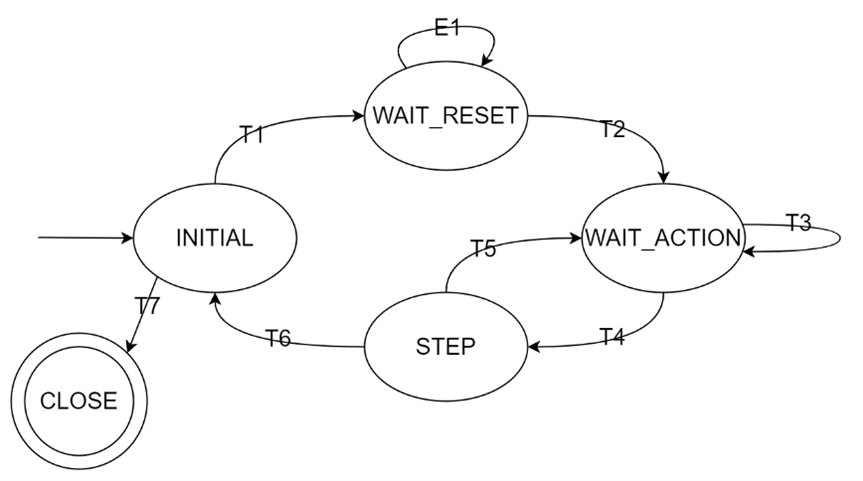
\includegraphics{images/aivle-gym-multi-dfa.png}
    \caption{aiVLE Gym Multi-agent Communication DFA}
    \label{fig:aivle-gym_dfa}
\end{figure}

\begin{enumerate}
    \item States: INITIAL, WAIT\_RESET, WAIT\_ACTION, STEP, CLOSE
    \item Initial state $q_0$: INITIAL
    \item Accept (terminal) states $F$: CLOSE
    \item Input symbols: method (e.g. reset/step/close) and other conditions
\end{enumerate}

To make this DFA a mathematically rigorous one, the domain of transition function needs to be the Cartesian product of input symbols and states. However, since there are many symbols and states involved, listing them exhaustively takes too much space. For the sake of simplicity, we omitted many self-transitioning paths - if transitioning condition is not satisfied, we assume there's a self-transition path. ``Meaningful'' transitions are described below:

\begin{itemize}
    \item T1
    \begin{itemize}
        \item condition: method is "reset"
        \item artifact: reset the underlying base Gym environment, label this agent as already reset, save this agent's router ID
    \end{itemize}
    \item E1
    \begin{itemize}
        \item condition: method is "reset" and this sender hasn't reset before
        \item artifact: label this agent as already reset, save this agent's router ID, trigger an input symbol of "E1" (This trigger is conceptually equivalent immediately checking if we can transit to the next state. Details can refer to the implementation.)
    \end{itemize}
    \item T2
    \begin{itemize}
        \item condition: input symbol of "E1", all agents are labelled as have reset
        \item artifact: send initial observation to all agents, clear reset labels, clear router ID mappings
    \end{itemize}
    \item T3
    \begin{itemize}
        \item condition: method is "step"
        \item artifact: label this agent as already stepped, save this agent's router ID, save this agent's action, trigger an input symbol of "T3"
    \end{itemize}
    \item T4
    \begin{itemize}
        \item condition: input symbol of "T3", all agents are labelled as have stepped
        \item artifact: step forward in the base environment, send observation/reward/done/info to all agents, trigger an input symbol of "T4"
    \end{itemize}
    \item T5
    \begin{itemize}
        \item condition: input symbol is "T4", some of the agents still have ongoing episode
        \item artifact: clear "have stepped" labels on all agents, clear router ID mappings
    \end{itemize}
    \item T6
    \begin{itemize}
        \item condition: input symbol is "T4", none of the agents still have ongoing episode
        \item artifact: same as T5
    \end{itemize}
    \item T7
    \begin{itemize}
        \item condition: method is "close"
        \item artifact: close the underlying environment
    \end{itemize}
\end{itemize}

By implementing this DFA carefully, the multi-agent judge environment abstract base class is capable of handling any order of incoming agent requests. Most importantly, agent-side can expect responses synchronously therefore keep all their expectations about a normal single-agent Gym environment. Note that these intricate details are not of users' (both the agent author and environment author) concern. The environment author only needs to provide implementations for the abstract methods and our library will handle the rest.
\chapter{aiVLE Worker Design}
\label{appendix:aivle-worker}

\section{Comparison of Mainstream Security Solutions}
\label{as:comparison-of-security-solutions}

There are several ``asterisks'' to the claims listed in Table~\ref{tab:security-solutions}, which we are going to address in detail in this appendix section. 

First, by ``rootless'' we meant no root privilege is required \emph{after} the initial setup. All solutions listed, including Firejail, requires root privilege to install. However, using it afterwards does not require root privilege.

Second, why in Docker and Podman is considered to be ``rootless'', but we still say that they ``prevent the GPU from being shared by any other container with root access''? It is because both Docker and Podman have a ``rootless mode'', which allows application to run without root access, however it also forces the GPU to run on rootless mode. Take Docker as an example, Docker Engine 20.10 introduced \href{https://docs.docker.com/engine/security/rootless/}{rootless Docker daemon}. But just like Podman, in rootless mode to make NVidia container runtime work you still need to \href{https://www.redhat.com/en/blog/how-use-gpus-containers-bare-metal-rhel-8}{set no-cgroups = true}, therefore \href{https://github.com/NVIDIA/nvidia-container-runtime/issues/85}{breaks root access from containers}.

Third, the ``level of isolation'' of Firejail is labelled as ``medium'' in the table. In fact, Firejail security entirely relies on how strict the security profile is – by default there is no restriction at all. The recommended approach according to \href{https://firejail.wordpress.com/documentation-2/building-custom-profiles/}{Firejail documentation} is to start with a strictest possible profile, then gradually white-listing features until the application inside the sandbox works fine. Since the full lockdown provided by Firejail is very strict, we consider it as a ``secure-enough'' alternative.

Lastly, VM is labelled to have no GPU support in the table. However, VM does support \textbf{exclusive} GPU access by technologies such as \href{https://docs.fedoraproject.org/en-US/Fedora/13/html/Virtualization_Guide/chap-Virtualization-PCI_passthrough.html}{PCI passthrough}. Exclusivity is the keyword here: we require the solution to work on shared instances, therefore we ignore such infeasible solutions.


% \chapter{Proofs}
% In this appendix, we present alternate, longer, but more interesting proof 
% of correctness of our algorithm.  This proof is based on induction and proof
% by contradiction.
\end{document}
